\chapter{Usando Flexbox}

\begin{flushright}
  \textit{
    Aquele que não luta pelo futuro que quer, \\
    deve aceitar o futuro que vier
  } \\
  
  \textbf{Autor desconhecido}
\end{flushright}

\section{Terminologias básicas}

Algumas terminologias básicas apresentadas neste capítulos devem ser entendidas para que haja um bom aproveitamento do conteúdo que será repassado. As duas são: \textbf{Containers} e \textbf{Itens}

A ideia de um container é muito semelhante a dos containers de navíos. Ou seja, um objeto que tem como única função conter outros objetos. Já os itens são, como você já deve ter imaginado, os objetos contidos dentro do container. 

\begin{figure}[H]
  \centering
  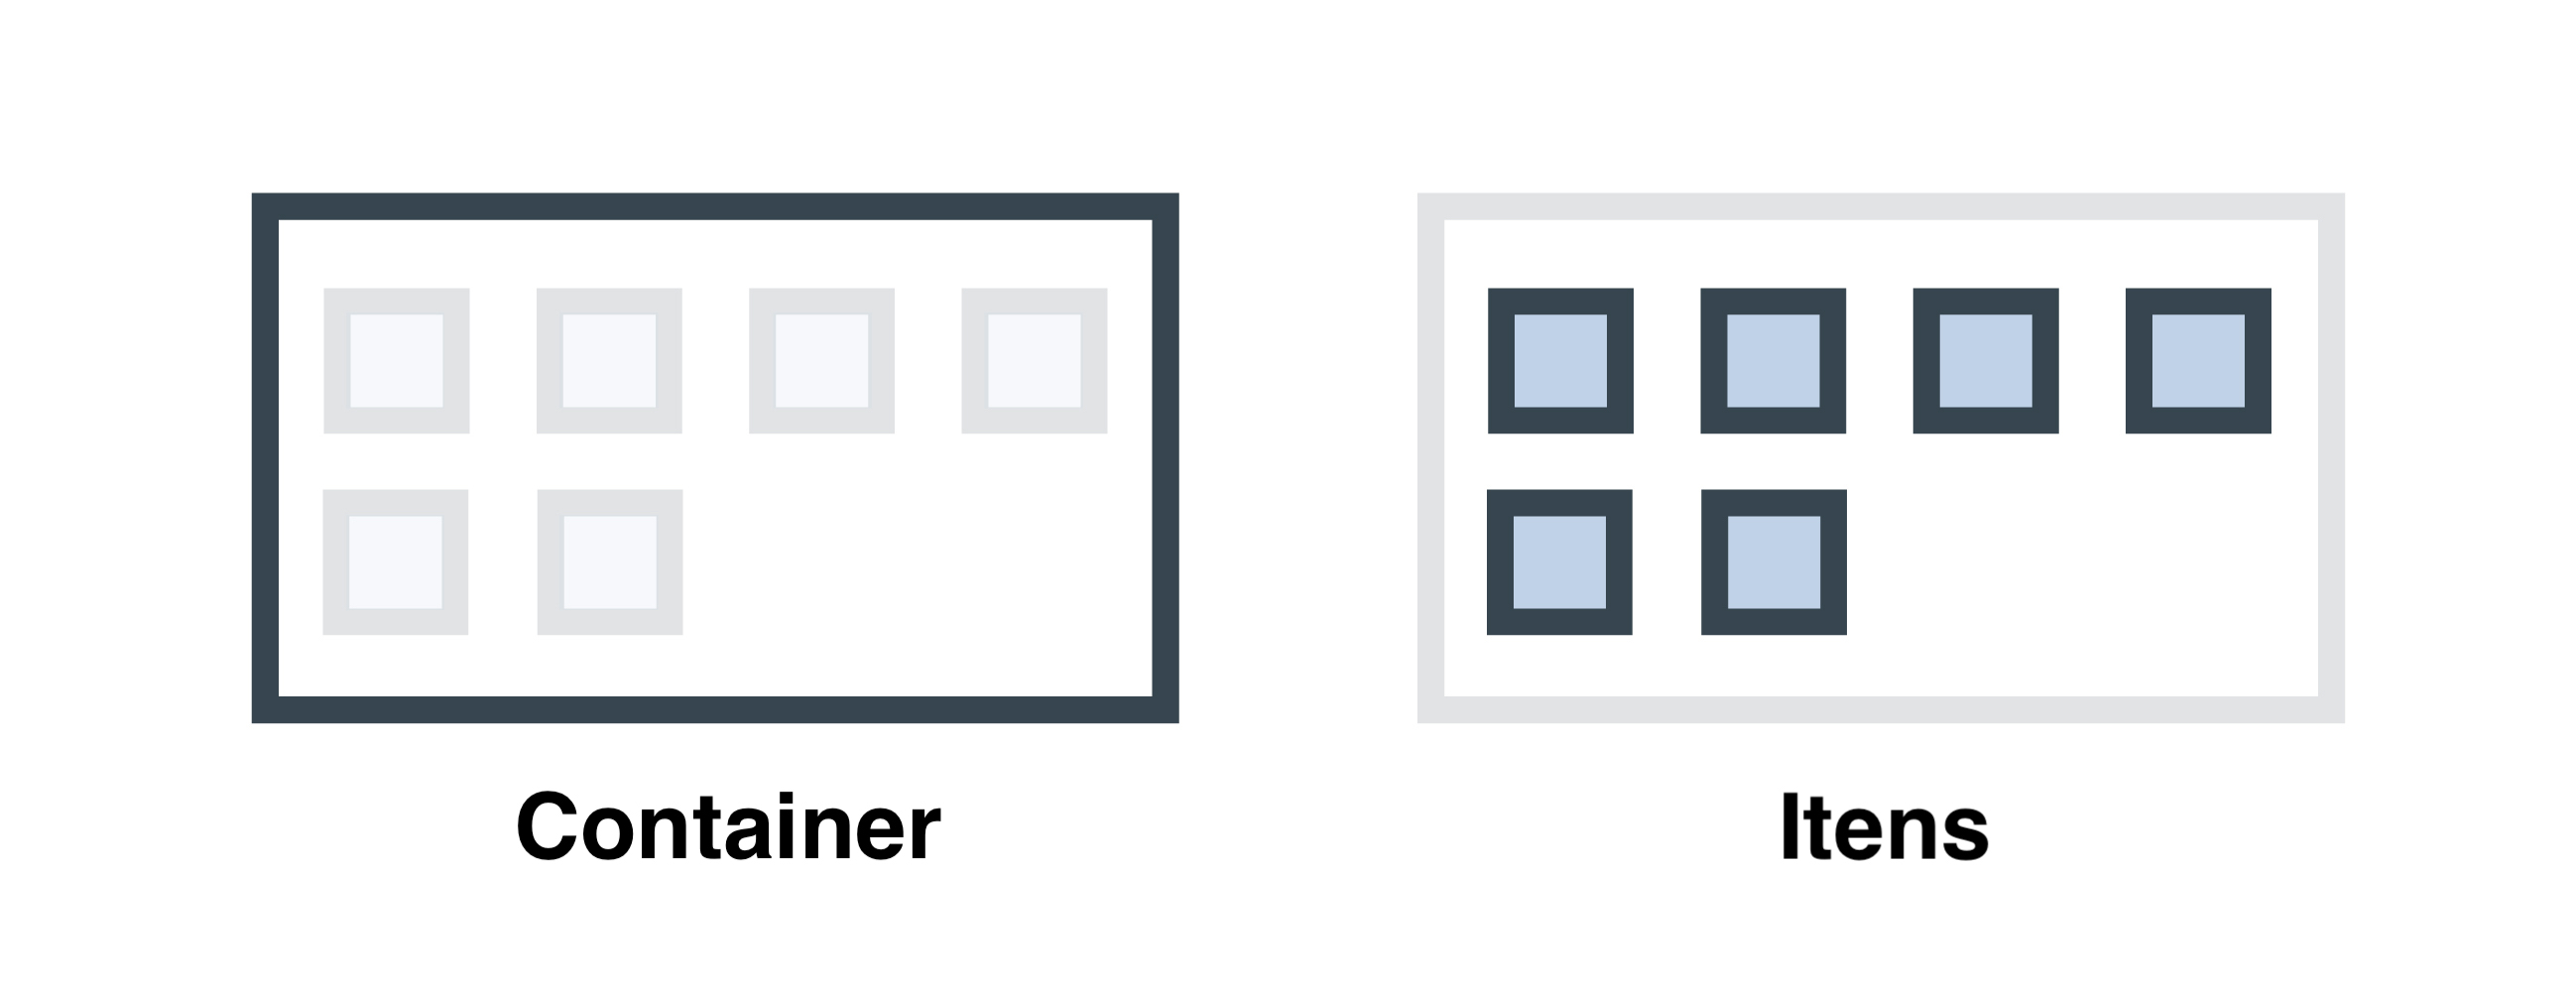
\includegraphics[scale=0.12]{imagens/container-itens.jpeg}
  \caption{Modedo do flexbox}
  \legend{Fonte: \cite{Buytaert2018} adaptado pelo autor}
  \label{fig:model-flexbox}
\end{figure}

\section{Propriedades do Flexbox}

Nesta sessão vamos aprender algumas propriedades do FlexBox. Fiquei ciente que nem todos os códigos, principalmente o de estilo, são descritos no texto abaixo mas apenas os códigos básicos para o entendimento dos conceitos apresentados.

\subsection{Flex Container}

A primeira propriedade que veremos é a \textbf{flex-container}. Esta propriedade define qual será o nosso container. Para tanto apenas utilizamos a propriedade \textbf{display} com o valor \textbf{flex}. Desta forma, passamos a nosso componente que ele deve se comportar de acordo com a diretiva, ou seja, organizar os itens de forma horizontal.

\begin{lstlisting}
  .flex-container {
    display: flex;
  } 
\end{lstlisting}

\begin{lstlisting}
  <div class="flex-container">
    <div>1</div>
    <div>2</div>
    <div>3</div>
  </div>
\end{lstlisting}

Como resultado apresentado na Figura \ref{fig:flex-container}, obtemos os itens organizados de forma horizontal. Lembrando novamente que o resultado contém estilos e formatação, sendo que o código acima demostra apenas as propriedades básicas sem estilo.

\begin{figure}[H]
  \centering
  
\includegraphics[scale=0.5]{imagens/flex-container.png}
  \caption{Flex Container}
  \legend{Fonte: O autor}
  \label{fig:flex-container}
\end{figure}

\subsection{Flex Direction}

A propriedade \textbf{flex-direction} define em qual direção o conteiner deseja empilhar os itens. O valor \textbf{column} empilha os itens verticalmente (de cima para baixo):

\begin{lstlisting}
  .flex-container {
    display: flex;
    flex-direction: column;
  } 
\end{lstlisting}

Como resultado apresentado na Figura \ref{fig:flex-direction-column} obtemos os itens em forma de pilha, organizados de cima para baixo abedecendo o formato de colunas, como passado na propriedade citada.

\begin{figure}[H]
  \centering
  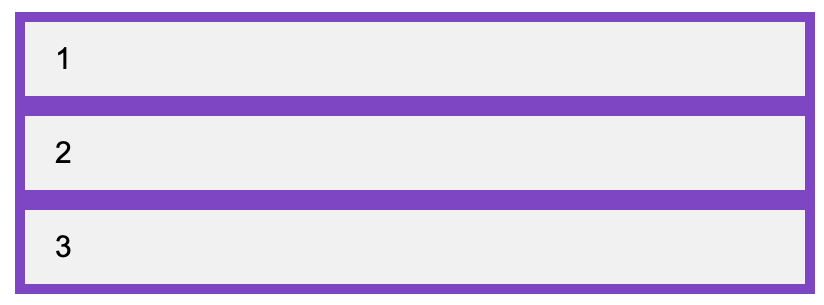
\includegraphics[scale=0.4]{imagens/flex-direction-column.png}
  \caption{Flex direction column}
  \legend{Fonte: O autor}
  \label{fig:flex-direction-column}
\end{figure}

Já o valor \textbf{column-reverse} empilha os itens verticalmente também. Contudo de baixo para cima:

\begin{lstlisting}
  .flex-container {
    display: flex;
    flex-direction: column-reverse;
  } 
\end{lstlisting}

Resultado: 

\begin{figure}[H]
  \centering
  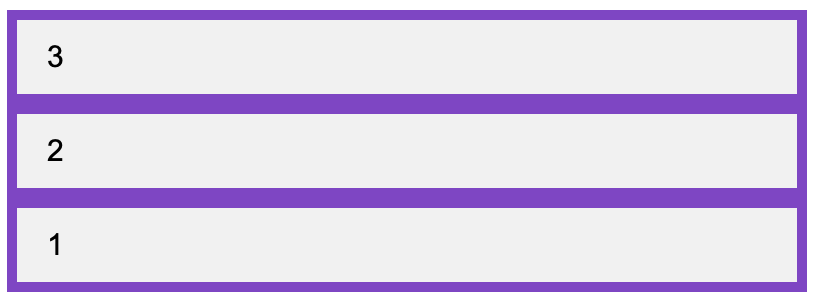
\includegraphics[scale=0.4]{imagens/flex-direction-column-reverse.png}
  \caption{Flex direction column reverse}
  \legend{Fonte: O autor}
  \label{fig:model-flexbox}
\end{figure}

Muito semelhante ao \textbf{column} ou o \textbf{column-reverse} o valor \textbf{row} e o \textbf{row-reverse} executam função muito parecidas mas os itens são enfileirados:

\begin{lstlisting}
  .flex-container {
    display: flex;
    flex-direction: row;
  } 
\end{lstlisting}

Resultado: 

\begin{figure}[H]
  \centering
  
\includegraphics[scale=0.4]{imagens/flex-direction-row.png}
  \caption{Flex direction row}
  \legend{Fonte: O autor}
  \label{fig:model-flexbox}
\end{figure}

\begin{lstlisting}
  .flex-container {
    display: flex;
    flex-direction: row-reverse;
  } 
\end{lstlisting}

Resultado: 

\begin{figure}[H]
  \centering
  
\includegraphics[scale=0.4]{imagens/flex-direction-row-reverse.png}
  \caption{Flex direction roe reverse}
  \legend{Fonte: O autor}
  \label{fig:model-flexbox}
\end{figure}

\subsection{Flex wrap}

A propriedade \textbf{flex-wrap} especifica se os itens devem ser agrupados ou não. Os exemplos abaixo contém 12 itens, os quais podem ou não ser agrupados mediante ao tamanho do container pai.

\begin{lstlisting}
  .flex-container {
    display: flex;
    flex-wrap: wrap;
  } 
\end{lstlisting}

Resultado: 

\begin{figure}[H]
  \centering
  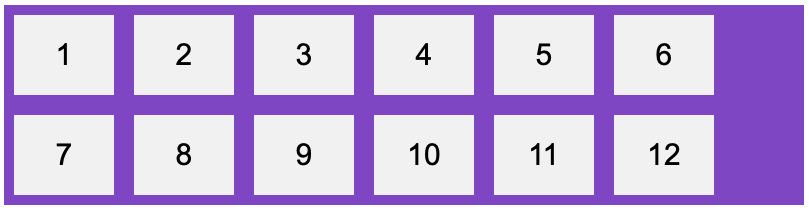
\includegraphics[scale=0.4]{imagens/flex-wrap.png}
  \caption{Flex wrap}
  \legend{Fonte: O autor}
  \label{fig:model-flexbox}
\end{figure}

\begin{lstlisting}
  .flex-container {
    display: flex;
    flex-wrap: nowrap;
  } 
\end{lstlisting}

Resultado: 

\begin{figure}[H]
  \centering
  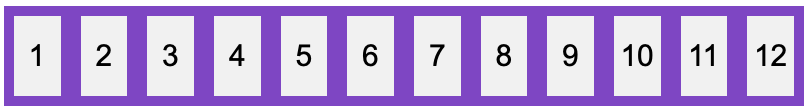
\includegraphics[scale=0.4]{imagens/flex-nowrap.png}
  \caption{Flex nowrap}
  \legend{Fonte: O autor}
  \label{fig:model-flexbox}
\end{figure}

O \textbf{flex-wrap} também possui o seu reverso. Logo, usando a propriedade \textbf{wrap-reverse} os itens são empilhados na ordem inversa.

\begin{lstlisting}
  .flex-container {
    display: flex;
    flex-wrap: wrap-reverse;
  } 
\end{lstlisting}

Resultado: 

\begin{figure}[H]
  \centering
  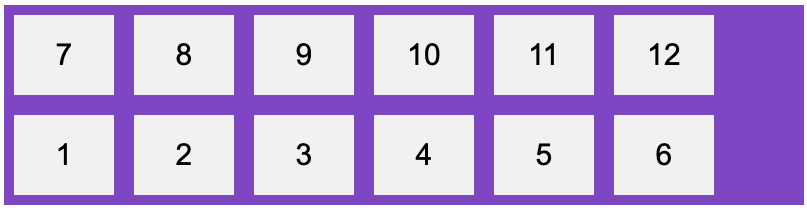
\includegraphics[scale=0.4]{imagens/flex-wrap-reverse.png}
  \caption{Flex wrap reverse}
  \legend{Fonte: O autor}
  \label{fig:model-flexbox}
\end{figure}

\subsection{Alinhamento de itens na horizontal}

A propriedade \textbf{justify-content} é usada para alinhar os itens em um container, seus valores podem ser \textbf{center}, \textbf{flex-start} e \textbf{flex-end}:

\begin{lstlisting}
  .flex-container {
    display: flex;
    justify-content: center;
  } 
\end{lstlisting}

Resultado: 

\begin{figure}[H]
  \centering
  
\includegraphics[scale=0.4]{imagens/justify-content-center.png}
  \caption{Justify content center}
  \legend{Fonte: O autor}
  \label{fig:model-flexbox}
\end{figure}

O valor \textbf{flex-start} alinha os itens no início do container (este é o padrão):

\begin{lstlisting}
  .flex-container {
    display: flex;
    justify-content: flex-start;
  } 
\end{lstlisting}

Resultado: 

\begin{figure}[H]
  \centering
  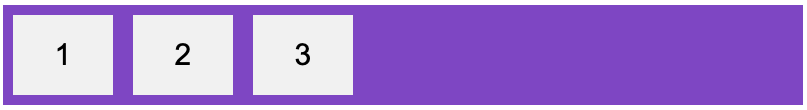
\includegraphics[scale=0.4]{imagens/justify-content-flex-start.png}
  \caption{Justify content Flex Start}
  \legend{Fonte: O autor}
  \label{fig:model-flexbox}
\end{figure}

O valor \textbf{flex-end} alinha os itens no final do conteiner:

\begin{lstlisting}
  .flex-container {
    display: flex;
    justify-content: ;
  } 
\end{lstlisting}

Resultado: 

\begin{figure}[H]
  \centering
  
\includegraphics[scale=0.4]{imagens/justify-content-flex-end.png}
  \caption{Justify content Flex End}
  \legend{Fonte: O autor}
  \label{fig:model-flexbox}
\end{figure}

\subsection{Alinhamento de itens na vertical}

Ao trocarmos a propriedade \textbf{justify-content} por \textbf{align-items} obtemos a possibilidade do alinhamento de itens na verticial sendo que os valores continuam os mesmos do \textbf{justify-content}

\begin{lstlisting}
  .flex-container {
    display: flex;
    align-items: center;  /* flex-start  ou flex-end */
  } 
\end{lstlisting}

\section{Conclusão}

Podemos aprender neste capítulo algumas das propriedades que vamos utilizar durante o curso. Contudo, Flexbox contém outras propriedades que podem ajudar no desenvolvimento de projetos de forma simples. Assim, caso haja alguma dúvida ou necessite de alguma propriedade que não foi listada neste texto, recomendo este link (https://origamid.com/projetos/flexbox-guia-completo/) o qual contém todos as  propriedade juntamente com exemplos de seu uso.